\documentclass[10pt]{article}

\usepackage{spheric}
%%%TITLE
\title{Water Hammer Analysis Using SPH in Density Summation Form}
\date{}

%%AFFILIATIONS

\author[1]{Darcy Q. HOU$^\dagger$}
\author[2]{Chunying HUANG}
\author[3]{Manli WANG}
\author[4]{Huanfeng DUAN}

\affil[1]{School of Computer Science and Technology, Tianjin University, China}
\affil[2]{School of Computer Software, Tianjin University, China}
\affil[3]{School of Municipal and Environmental Engineering, Shandong Jianzhu University, China}
\affil[4]{Department of Civil and Environmental Engineering, The Hong Kong Polytechnic University, Hong Kong}
\affil[$\relax$]{\email{\dagger}{qhou@tju.edu.cn}}


%%DOCUMENT
\begin{document}

\maketitle

%\SelectedTopics{}

%%PLEASE PUT YOUR ABSTRACT HERE
\begin{abstract}
Water hammer in fluid piping systems can induce serious damages to hydraulic machinery, piping and supports, and it should be prevented in practice. Therefore, numerical analysis of this phenomenon plays an important role in hydraulic engineering. The discontinuity of the solution, however, results in various difficulties for numerical methods. 

We had successfully simulated the water hammer problem with both the original smoothed particle hydrodynamics (SPH) method \cite{hou2016meshless} and its correction, the corrective smoothed particle method (CSPM) \cite{hou2012simulating}. Comparing with traditional SPH, boundary conditions can be efficiently imposed in CSPM without using any fictitious or ghost particles. In \cite{hou2016meshless,hou2012simulating} together with momentum equation, time dependent continuity equation is solved. 

Based on the fact that the density evolution in summation form works much better than the continuity equation in shock tube problems, we explore here the possibility of simulating water hammer problem by solving the SPH density summation equation and momentum equation. Numerical results shown in Fig. \ref{fig:49} indicate that promising results can be obtained if the equation of state is properly treated. In addition, as long as the CFL condition is satisfied, time stepping and variable smoothing length have almost no effect on the numerical results (see Fig. \ref{fig:49}).

\begin{figure}[!htb]
\centering
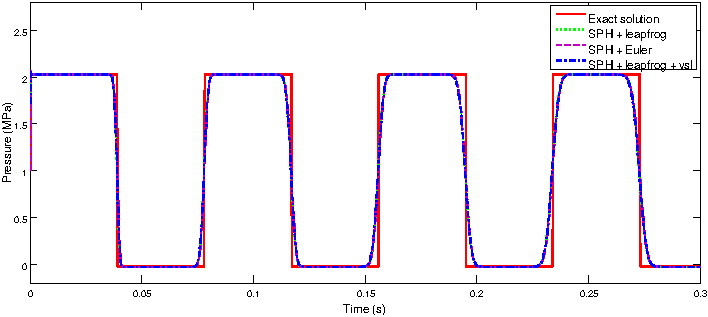
\includegraphics[width=0.95\textwidth]{49-1.pdf}
\caption{Pressure traces at downstream valve solved by SPH in density summation form with different time stepping and variable smoothing length.}\label{fig:49}
\end{figure}

\end{abstract}


%%THE END OF ABSTRACT

\addbib

\end{document}
